\subsection{Packet, Trace and Monitor}
\label{subsec:basic}

The observations of the DUT constitute packets sent and received at certain
timestamps.
%
Aspects of the protocol specification can be monitored using state machines
to validate the observations of the DUT.
%
In this section, we formally define these concepts.
%
More specifically, we use \textit{timed automata}~\cite{alur1994theory} to model
the expected behaviors of the DUT with correct protocol implementation.
%
A timed automata is a finite state machine with timing constraints on the
transitions: each transition can optionally start one or more timers, which can
later be used to assert certain events should be seen before or after the time
out event(s).
%
We use the term \textit{timed automata} and \textit{state machine}
interchangeably hereafter.

The input alphabet of the state machine is the finite set of all valid packets defined
by the protocol, denoted as $\mathbb{P}$. 
%
A packet is a binary string of finite number of bits, encoding interesting
protocol attributes such as \texttt{src}, \texttt{dest}, \texttt{type},
\texttt{flags}, and physical layer information, such as \texttt{channel},
\texttt{modulation}, etc.

Next, we define the \textit{observation} that corresponds to time-ordered
sequence of packets.
\begin{definition}
  \sloppy{%
    A \textit{packet trace} is a finite sequence of $(timestamp, packet)$ tuple:%
  }%
  \begin{align*}
    [(t_1, p_1), (t_2, p_2),\ldots,(t_n, p_n)]
  \end{align*}%
  where $t_i \in \mathbb{Z}^+$ is the \textit{discrete} timestamp and $p_i$ is the packet
  observed by the DUT at time $t_i$. The timestamps are strictly monotonically increasing,
  $t_i < t_{i+1}$ for $1 \le i < n$.
\end{definition}%

In addition to timestamp monotonicity, we also require that adjacent packets do
not overlap in time, $t_{i+1}-t_i > \text{\texttt{airtime}}(p_i)$ for $1 \le i
< n$, where \texttt{airtime()} calculates the time taken to transmit a packet
based on its size and modulation scheme.

We now formally define the monitor state machine that models the expected
behavior of the DUT and serves as the protocol specification.

\begin{definition}
  A protocol monitor state machine $S$ is an 6-tuple $\{\Sigma, \mathbb{S}, s_0, C, E, G\}$, where:
  \begin{itemize}
    \item $\Sigma = \mathbb{P}$ is the finite input alphabet.
    \item $\mathbb{S}$ is a non-empty, finite set of states. $s_0 \in
      \mathbb{S}$ is the initial state.
    \item $C$ is the set of clock variables. A \textit{clock variable} can be
      reset along any state transitions. At any instant, reading a clock
      variable returns the time elapsed since last time it was reset.
    \item $G$ is the set of clock constraints defined inductively by
      \begin{align*}
        g := true\ |\ c \le T\ |\ c \ge T\ |\ \neg g\ |\ g_1 \land g_2
      \end{align*}%
      where $c \in C$ is a clock variable and $T$ is a constant. Note that an
      transition can choose not to use clock guard by setting $g$ to be $true$.
    \item $E \subseteq \mathbb{S} \times \mathbb{S} \times \Sigma \times  G \times \mathscr{P}(C)$
      gives the set of transitions. $\langle s_i, s_j, p, g, C'\rangle \in E$
      represents that if the monitor is in state $s_i$, given the input tuple
      $(t, p)$ such that the clock variables satisfies the guard $g$, the
      monitor transits to state $s_j$ and reset the clocks in $C'$ to 0.
  \end{itemize}
  \label{def:sm}
\end{definition}

A tuple $(t_i, p_i)$ in the packet trace means the packet $p_i$ is presented to
the state machine at time $t_i$.
%
The monitor rejects a trace $Tr$ if there exists a prefix of $Tr$ such that all
states reachable after consuming the prefix have no valid transitions for the
next $(t, p)$ input.
%
Note that the input to the state machine, time and packet, are all
observable events in the medium.
%
Validating the internal events of the DUT is beyond the
scope of this paper.

Next, we give an example monitor state machine for the transmitter in 802.11
data transmission protocol.
%
Without loss of generality, we assume the DUT only
retransmits the packet at most once if the first transmission failed.
%
The state machine can be easily adapted to accommodate multiple retransmissions.

There are only three types of packets to consider in this case: $DATA_i$ denotes
a packet sent by the transmitter with sequence number $i$, $DATA'_i$ denotes the
retransmission of $DATA_i$, and $Ack$ is the acknowledgment packet sent by the
receiver.
%
The sequence number is within the range of $[0, N)$.

\begin{figure}[t!]
  \centering
  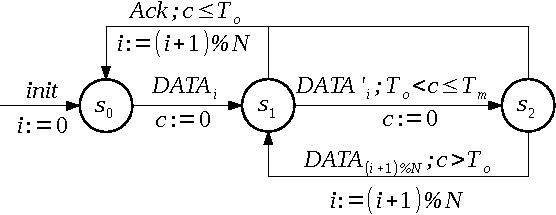
\includegraphics[width=0.45\textwidth]{./figures/dot11_tx_ta.pdf}
  \caption{\textbf{Transmitter Monitor State Machine for 802.11 Packet Transmission
  Protocol.}}
  \label{fig:dot11_tx_ta}
\end{figure}



The monitor state machine is illustrated in Figure~\ref{fig:dot11_tx_ta}, and
the main components are:

\begin{itemize}
  \item $\Sigma = \{DATA_i, DATA'_i, Ack\ |\ 0 \le i < N\}$.
    %
  \item Clock variables $C = \{c\}$. The only clock variable $c$ is
    used for acknowledgment time out.
    %
  \item Guard constraints $G = \{ c \le T_o, c > T_o, T_o < c \le T_m\}$.
    $T_o$ is the acknowledgment time out value, and $T_m >
    T_o$ is the maximum delay allowed before the retransmission packet gets
    sent. $T_o$ can be arbitrary large but not infinity in order to check the
    liveness of the DUT.
\end{itemize}

To succinctly present the state machine, we use an internal variable $i$ to keep
track of the next sequence number.
%
One can easily eliminate this variable and
use only different states for different sequence numbers.
%
Therefore, this state machine is consistent with Definition~\ref{def:sm}.

The sequence number $i$ is initialized to 0 when the state machine is
initialized.
%
At state $s_0$, the monitor expects to see a $DATA_i$ packet.
%
It transits to $s_1$ when such event happens and resets acknowledgment timer $c$ along the transition.
%
At state $s_1$, two valid events can happen: either the DUT receives $Ack$ packet
within time $T_o$ ($s_1\rightarrow s_0$), or the DUT sends $DATA'_i$ after $T_o$
but before $T_m$ ($s_1 \rightarrow s_2$).
%
Similarly at state $s_2$, either the DUT receives $Ack$ within time $T_o$ ($s_2
\rightarrow s_0$), or otherwise the DUT concludes that the previous transmission
failed and continues to transmit the next packet $s_2\rightarrow s_1$.

The monitor state machine defines a \textit{timed language} $L$ which consists
all valid packet traces that can be observed by the DUT.
%
We now give the
definition of protocol \textit{compliance} and \textit{violation}.

\begin{definition}
  Suppose $\mathbb{T}$ is the set of all possible packet traces collected from
  DUT, and $S$ is the state machine specified by the protocol. The DUT
  \textit{violates} the protocol specification if there exists an
  packet trace $Tr \in \mathbb{T}$ such that $S$ rejects $Tr$.
  Otherwise, the DUT is \textit{compliant} with the specification.
\end{definition}

The focus of this paper is to determine whether a \textit{given} $Tr$ is
evidence of a violation.
%
We acknowledge that determining \textit{compliance} is a more challenging
problem, as it requires enumerating every possible trace in $\mathbb{T}$, which
is probably infinite.
